%Centralizar verticalmente.
\newenvironment{midpage}{\vspace*{\fill}}{\vspace*{\fill}}
%Centralizar horizontalmente.
\newenvironment{midline}{\hspace*{\fill}}{\hspace*{\fill}}
\documentclass[12pts]{article}
\usepackage[utf8]{inputenc} 
\title{
	Prática de Eletrônica Digital 1 - (119466)
	\singlespacing
		Turma E (Unb - Gama)
	\singlespacing
	\begin{midpage}
	\begin {large}
		Relatório Experimento 3 
		\singlespace
		Circuitos Somadores e Subtratores
	\end {large}
	\end{midpage}
}
\date{Setembro 15, 2016}
\usepackage{indentfirst}
\usepackage{setspace}
\usepackage{verbatim}
\usepackage[pdftex]{hyperref}
\usepackage{graphicx}
\begin{document}
\maketitle	
%\vspace{100 mm}
\begin{center}

\begin{tabular}{|c|l|r|}
\hline
Nome & Matrícula & Assinatura\\
\hline
Arthur Temporim & 14/0016759 & \\
\hline	
Eduardo Nunes & 14/0056189 & \\
\hline	
\end{tabular}

\end{center}


\newpage

\section{Sumário}

\begin{itemize}
	\item Introdução
	\singlespacing
	\item Experimentos
	\singlespacing
	\item Discussão
	\singlespacing
	\item Conclusões 
	\singlespacing
	\item Referências Bibliograficas
	\singlespacing
	%\item Diagramas esquemáticos
\end{itemize}

\newpage


\section{Introdução}
\iffalse
Introdução, indicando a delimitação do tema, apresentando a justificativa descrevendo o propósito do relatório.
\fi
	Neste relatório é apresentado os resultados dos 3 experimentos realizados na aula da prática da eletrônica digital 1.
	São apresentados nos três experimentos a imagem do diagrama do circuito e a saída em forma de onda. Todos os experimentos foram realizados utilizando a ferramenta \textit{Ise design suite}.

\section{Experimentos}
\iffalse
Parte Experimental, descrevendo os passos realizados, dificuldades e soluções para os problemas encontrados. Aqui, deve-se apresentar uma descrição dos resultados encontrados em forma de figuras, gráficos e tabelas.
\fi

\textbf{Experimento 01}
\singlespacing
	O primeiro experimento tratou-se da realização de um circuito de complemento de 1 com 4 bits de entrada. Abaixo as imagens, respectivamente, são: Diagrama do circuito e a saída obtida em forma de onda.

\begin{figure}[!htb]
  \centering
  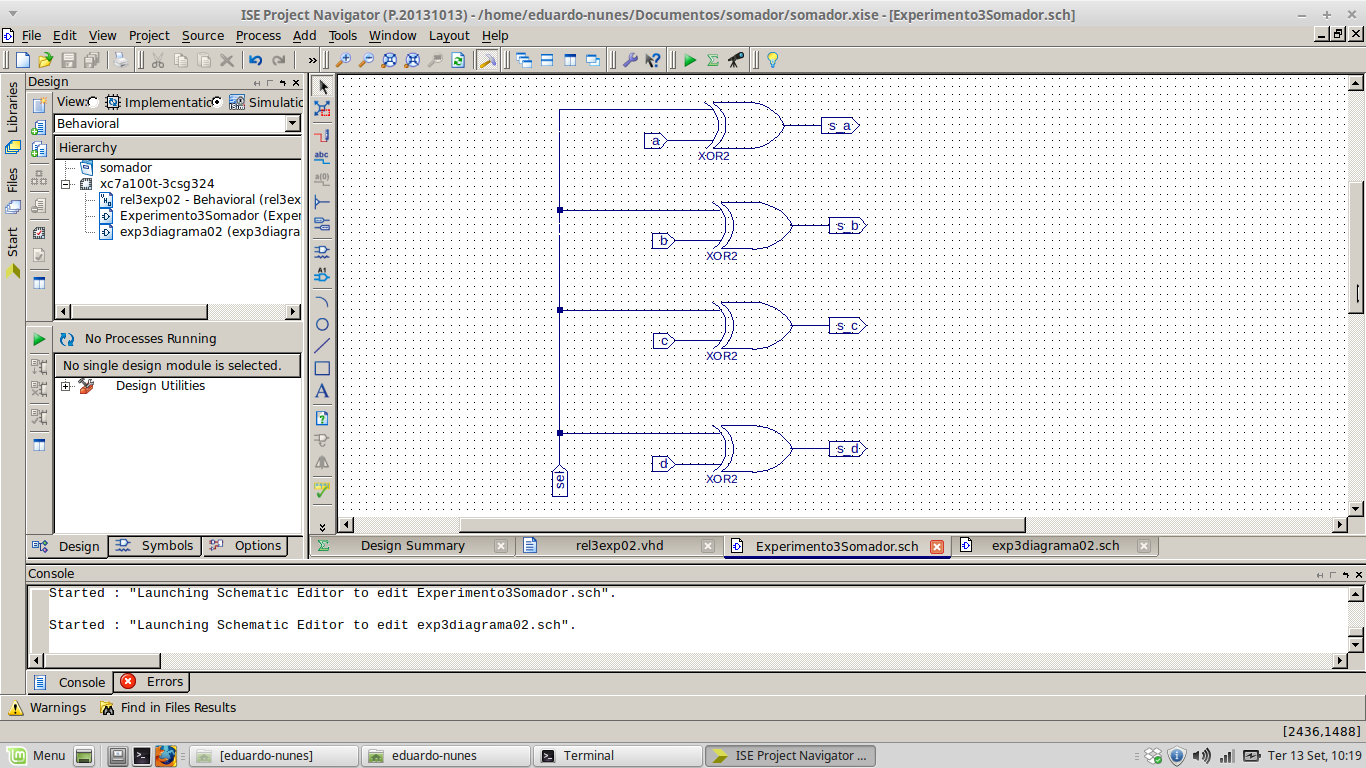
\includegraphics[scale=0.2]{img/complemento01.png}
  \caption{Diagrama do circuito complemento de 1 de 4 entradas - Ise Design Suite 14.7}
  \label{figRotulo}
\end{figure}

\begin{figure}[!htb]
  \centering
  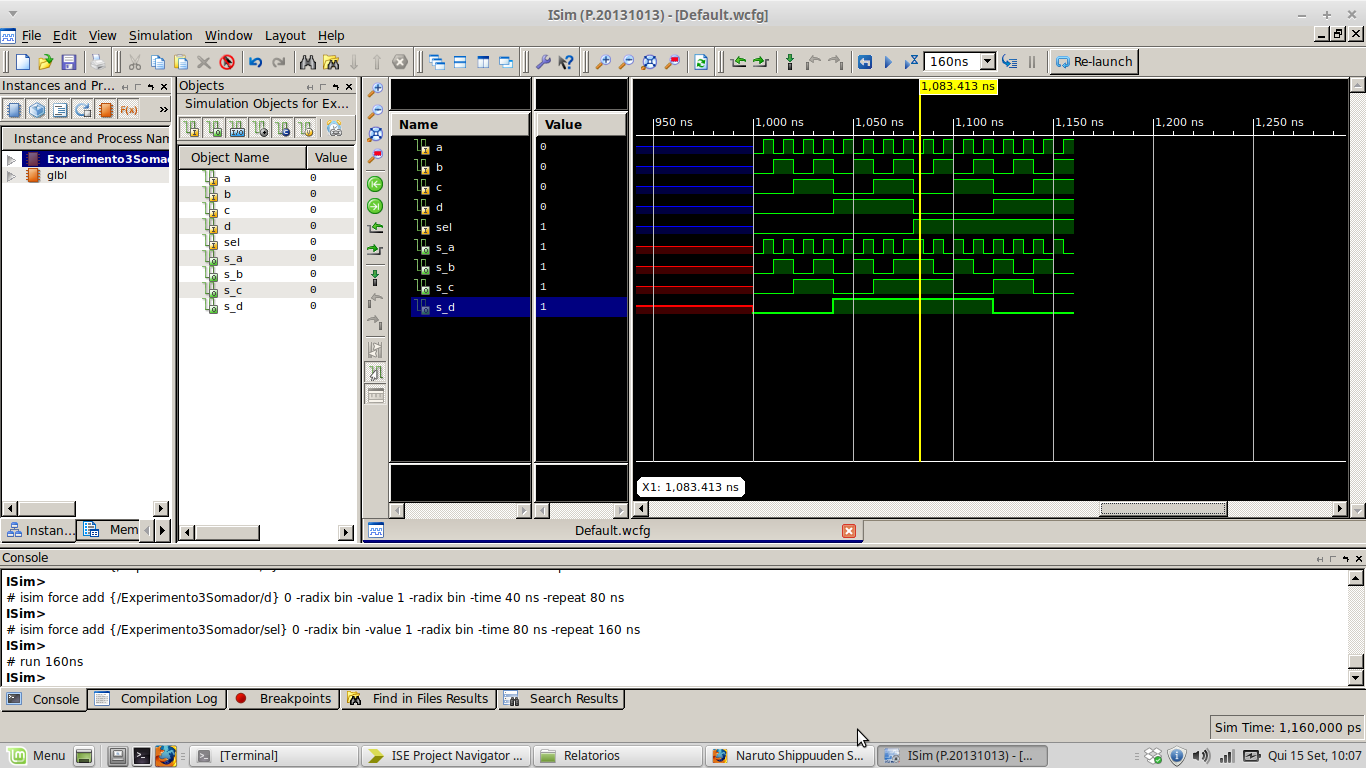
\includegraphics[scale=0.2]{img/saidaComplemento01.png}
  \caption{Diagrama de ondas do complemento de 1 de 4 entradas - Ise Design Suite 14.7}
  \label{figRotulo}
\end{figure}
\newpage

\textbf{Experimento 02}
\singlespacing
O segundo experimento tratou-se da realização de um circuito somador com 4 bits de entrada. As simulações e saídas estão representadas nas imagens a abaixo:


\begin{figure}[!htb]
  \centering
  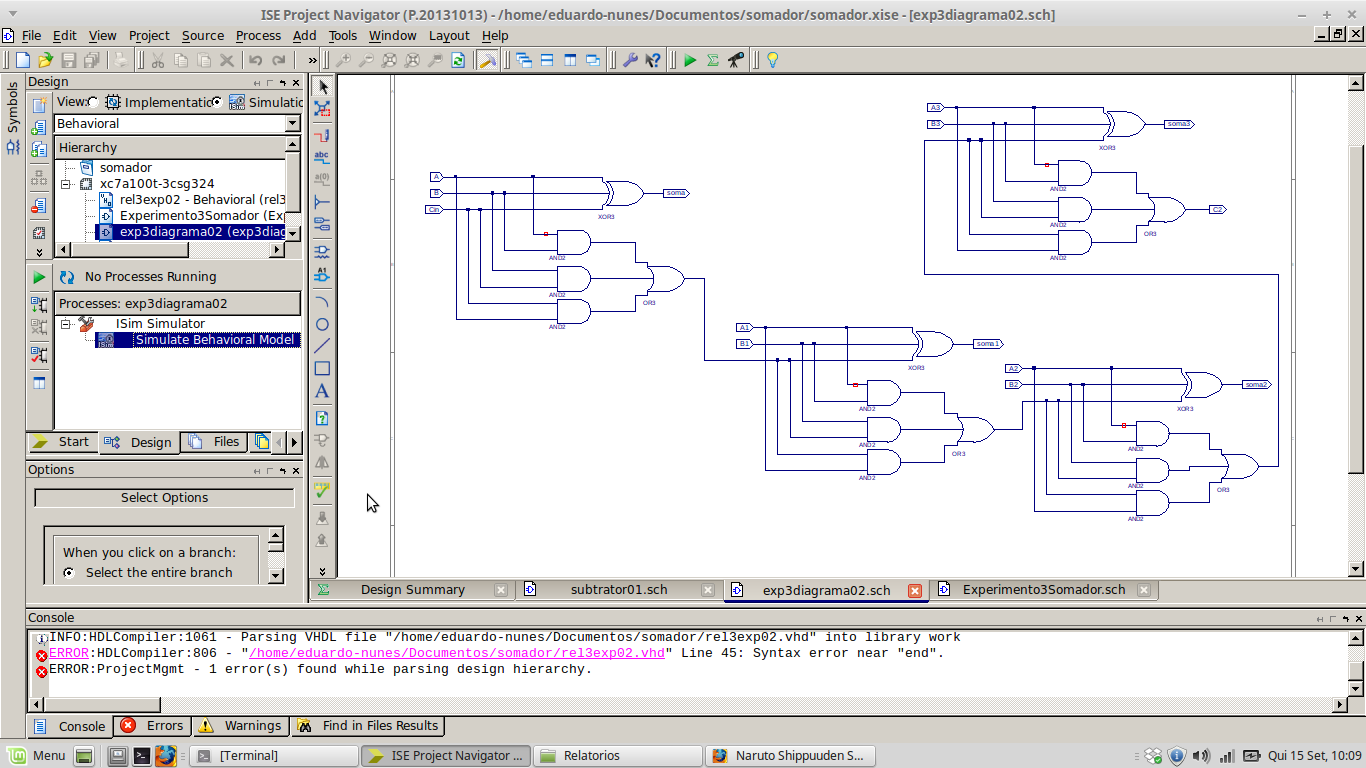
\includegraphics[scale=0.2]{img/somadorDefinitivo.png}
  \caption{Diagrama do circuito somador - Ise Design Suite 14.7}
  \label{figRotulo}
\end{figure}

\begin{figure}[!htb]
  \centering
  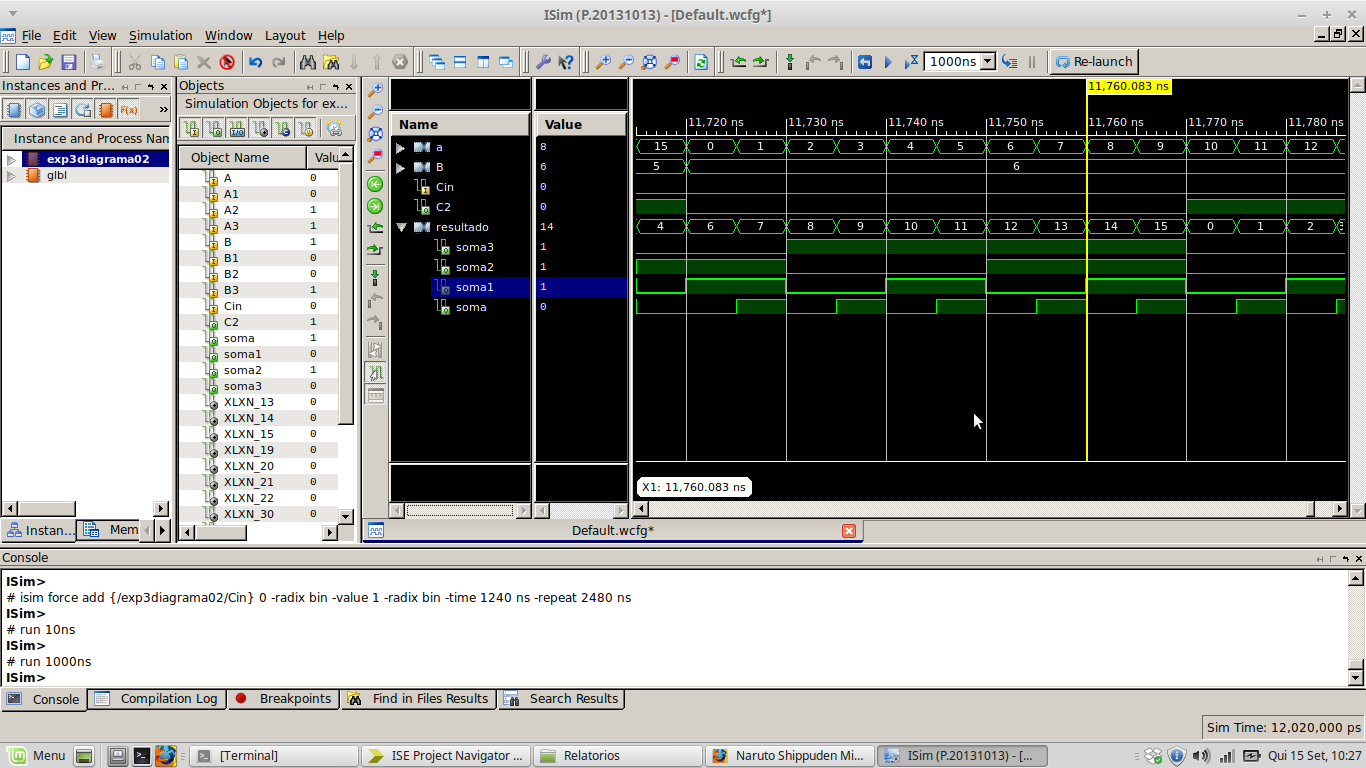
\includegraphics[scale=0.2]{img/saidaSomador}
  \caption{Diagrama de ondas somador - Ise Design Suite 14.7}
  \label{figRotulo}
\end{figure}

\newpage

\textbf{Experimento 03}
\singlespacing
O terceiro experimento tratou-se da realização de um circuito com 4 bits de entrada na qual a partir de uma chave de seleção determinava se o circuito somaria ou subtraria os valores de entrada. As simulações e saídas estão representadas nas imagens a abaixo:

\begin{figure}[!htb]
  \centering
  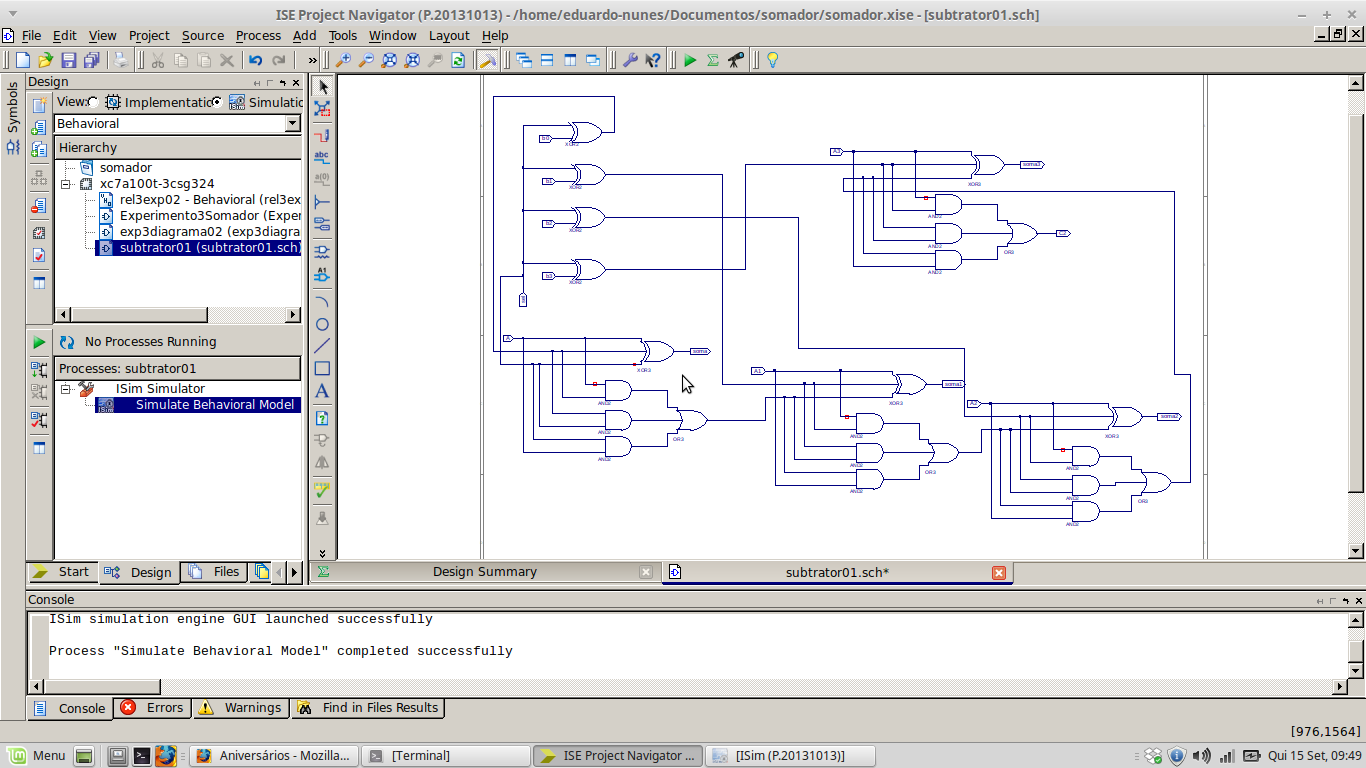
\includegraphics[scale=0.2]{img/subtrator}
  \caption{Diagrama do circuito 01 - Ise Design Suite 14.7}
  \label{figRotulo}
\end{figure}

\begin{figure}[!htb]
  \centering
  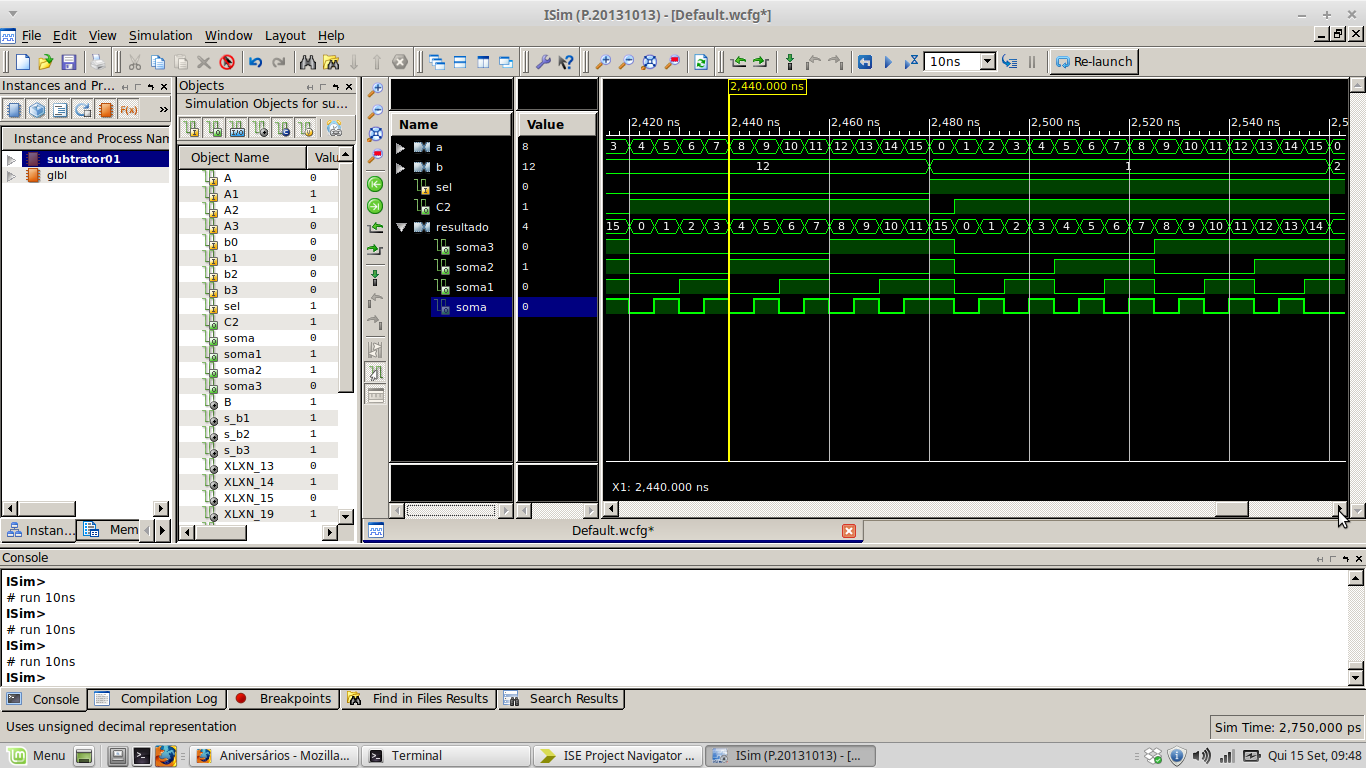
\includegraphics[scale=0.2]{img/subtratorSaida.png}
  \caption{Diagrama de ondas 01 - Ise Design Suite 14.7}
  \label{figRotulo}
\end{figure}

\newpage


\section{Discussão}
\iffalse
Discussão sobre os resultados encontrados, comentando detalhadamente as medições realizadas e dando a devida interpretação destas, informando se os objetivos da experimento foram alcançados. Esta é uma das partes mais importantes do relatório: aqui, há oportunidade para expressar os conhecimentos adquiridos na prática e fazer a interrelação com os fundamentos teóricos.
\fi

	Com a realização deste experimento foi possível adquirir conhecimento a respeito de sistemas somadores e subtratores. Todas os resultados apresentados nas saídas dos 3 experimentos foram de acordo com o esperado.

\section{Conclusões}
\iffalse
Conclusões, mostrando os êxitos e eventuais problemas encontrados na realização do experimento, indicando as limitações, apresentando recomendações e/ou sugestões.
\fi

	Neste terceiro relatório foi possível realizar todas as atividade com êxito porém houve dificuldade na hora de depurar o resultado das saídas pois havia números que não correspondiam ao valor desejado. Porém depois foi entendido que este valores não correspondentes se referiam a overflows, tal que o valor que devia se apresentado não podia ser representadado em apenas 4 bits. Desta forma, foi possivel determinar e entender como interpretar estes valores.

\section{Referências Bibliográficas}
\iffalse
Referencias Bibliográficas, relacionadas e citadas de acordo com as normas da ABNT.
\fi
Prática de Eletrônica Digital I 2016.2 professores Henrique Marra Taira Menegaz,Leonardo Aguayo, Lourdes Mattos Brasil, Marcus Vinícius Chaffim Costa, Mariana Costa Bernardes Matias. UnB - FGA Agosto de 2015.

\iffalse
\section{Diagramas Esquemáticos}
Diagramas Esquemáticos. Todos os diagramas devem ser inseridos ao final do relatório em páginas separadas do texto, indicando a identificação do circuito, autor, revisor, versão e datas relevantes.
\fi
\newpage
\end{document}

%Exemplo de imagem
\iffalse
\begin{figure}[!htb]
  \centering
  \includegraphics[scale=0.3	]{nome_da_imagem}
  \caption{Descrição}
  \label{figRotulo}
\end{figure}
\fi

% Exemplo de tabela.
\iffalse
\begin{tabular}{|c|r|}
\hline
Material Utilizado & Quantidade\\
\hline
Cabo Banana-Banana & 2  \\
\hline
Fios de cobre & x \\
\hline
Cabo coaxial & 3  \\
\hline
CI 74HC00   & 1 \\
\hline
CI 74LS00   & 1 \\
\hline
Protoboard & 2 \\
\hline
Fonte de tensão MPL-3305M & 1 \\
\hline	
Multímetro Digital  & 1 \\
\hline
Gerador de funçoes iCEL modelo GV-2002 & 1 \\
\hline
Osciloscopio BK 2530 & 1 \\
\hline
\end{tabular}
\singlespacing
\fi
